\section{Results}
\label{891_2:sec:results}

\subsection{Age and Metallicity}
\label{891_2:sec:tZ}

The analysis methods described above allow us to measure $\tau_L$ and
$Z_L$ as a function of galactic radius and height. This parameter
space can yield powerful insights into the history and formation of
NGC 891, but first it is useful to examine the distribution of these
parameters on a galactic scale, as shown in Figure
\ref{891_2:fig:tauZ_hist}. In the left panel we see a multi-modal
distribution of $\tau_L$ that suggests multiple epochs of star
formation in NGC 891. We assign these epochs 4 rough age bins: the
most recent epoch of star formation at $\tau_L < \val{4.3}{Gyr}$, a
somewhat quiescent and relatively constant era of star formation from
$\val{4.3}{Gyr}\leq\tau_L < \val{6.6}{Gyr}$, and two distinct bursts
at $\val{6.6}{Gyr}\leq\tau_L < \val{8}{Gyr}$ and
$\val{8}{Gyr}\leq\tau_L$.

The distribution of $Z_L$ shown in the right panel of Figure
\ref{891_2:fig:tauZ_hist} also reveals multiple populations: the main
peak can be split into two sub-peaks that occupy $\val{0.5}{\Zsol}\leq
Z_L < \val{0.75}{\Zsol}$ and $\val{0.75}{\Zsol}\leq Z_L <
\val{0.95}{\Zsol}$. A higher metallicity tail extends the distribution
out to $\val{0.95}{\Zsol}\leq Z_L < \val{1.3}{\Zsol}$ with a distinct
super-metal-rich population at $Z_L \geq\val{1.3}{\Zsol}$.

Armed with the global distribution of stellar populations in $\tau_L$
and $Z_L$ we can now examine where the different ranges defined above
exist in NGC 891. Figure \ref{891_2:fig:rz_tZ} shows both $\tau_L$ and
$Z_L$ as a function of radius and height. In the left panel the trends
identified in Chapter \ref{chap:891_1} are immediately obvious: below
\val{0.4}{kpc} all of the populations are young (\val{< 6.6}{Gyr}),
the region where $0.4 < |z| \leq \val{1}{kpc}$ is a transition zone
where the age generally increases, and above \val{1}{kpc} the light is
dominated by the oldest populations.

Examining radial trends in $\tau_L$ yields an even more detailed
picture. In general, younger ages tend to be more concentrated toward
larger radii, which is consistent with the inside-out formation
scenario seen in Chapter \ref{chap:891_1} and the Milky Way
\citep{Bovy12,Hayden15}. Furthermore, for each of the age epochs
defined above and in Figure \ref{891_2:fig:rz_tZ} there is a clear
flaring in height at larger radii. What's more, this ``flare radius''
is larger for more recent epochs of star formation (i.e., increasing
galaxy age). In other words, each epoch of star formation forms a
flared disk and as the galaxy ages star formation (and the
corresponding flare) migrate to larger and larger radii. Thus the
galaxy disk as a whole can be thought of as a superposition of flared
disks that formed at different times. These results are remarkably
consistent with those of \citet{Martig14a}, who suggest this pattern can
be caused by minor interactions with small satellites and/or radial
migration \citep{Minchev12}.

Trends in $Z_L$ shown in the right panel of Figure
\ref{891_2:fig:rz_tZ} complement the trends in $\tau_L$. Firstly, the
lowest metallicities exist primarily at large heights (although there
is a locus of points at small heights and large radii), which matches
the general view that the old populations at large heights were formed
from pristine gas early in the history of NGC 891. Modifying this
simple picture is the fact that the majority of populations with
super-solar metallicities also exist at intermediate to large
heights. Below \val{\asim0.4}{kpc} most of our data are sub-solar. As
discussed below we suspect this trend in metallicity with height is
indicative of a transition from galactic self-enrichment to
inflow-dominated metallicity suppression.

This transition can be seen in the left panel of Figure
\ref{891_2:fig:MLWZ_rz_cut}, which reveals two distinct trends in
metallicity with height. For populations with $\tau_L >
\val{6.6}{Gyr}$ metallicity decreases with height, as expected from
the simple view that old stars are made from pristine gas and exist at
large heights. Populations younger that \val{\asim 6.6}{Gyr} show the
opposite trend; here metallicity sharply increases as a function of
height. If we consider height to broadly correspond to age (see Figure
\ref{891_2:fig:MLWA_rz_cut}) then the following picture emerges:
during the first few Gyr of its history NGC 891 was essentially a
closed-box; each generation of stars was enriched by the chemical
processing of gas by the generations that preceded it. Around
\val{6.6}{Gyr} ago, however, low-metallicity gas from outside the
galaxy started to infall onto the disk, and as the amount of pristine
gas increased the average metallicity of subsequent populations
decreased. Thus, the ``peak metallicity'' of NGC 891 occurred roughly
\val{6.6}{Gyr} ago. The right panel of Figure
\ref{891_2:fig:MLWZ_rz_cut} confirms this: at all radii the largest
values of $Z_L$ occur in populations where $\tau_L \approx
\val{6.6}{Gyr}$.

In addition to the locus of metal-poor stars at large radii and small
heights (i.e., the most recent star formation) we identify a second
locus of metal-poor stars at small radii and intermediate heights. In
the context of the history proposed above, this second population
likely corresponds to the oldest portion of the disk or
pseudo-bulge. This view is strengthened by Figure
\ref{891_2:fig:MLWA_rz_cut}, which clearly shows two very different
physical locations of populations with $Z_L < \val{0.5}{\Zsol}$.

Figure \ref{891_2:fig:MLWA_rz_cut} offers another view of the scenario
presented above. To first order, age increases with height, as
expected from Chapter \ref{chap:891_1}, and above \val{1}{kpc} the
average population age asymptotes to the oldest age (\val{\asim
  10}{Gyr}). As described in \S\ref{891_2:sec:sys_err} the specific
value of $\tau_L$ at the largest heights is dependent on the physical
assumptions made when constructing the models (i.e., the first stars
in the Universe formed \val{\asim 12}{Gyr} ago), but these assumptions
only modulate the actual value; the conclusion that the integrated
light is dominated by the oldest possible populations above
\val{1}{kpc} is valid regardless of the specific population age.

The enrichment history of NGC 891 is also visible in Figure
\ref{891_2:fig:MLWA_rz_cut}. The highest metallicity populations have
ages narrowly scattered around $\tau_L \approx \val{6.6}{Gyr}$ (bottom
panels), which is exactly the age of ``peak metallicity'' identified
above. As metallicity decreases there is an increasing level of
bifurcation in age, representing the two epochs of metal-poor star
formation: the first, at large heights and small radii, corresponds to
the first stars formed in NGC 891. The second, at small heights and
large radii, corresponds to recent star formation that is drawing from
metal-poor gas that has been infalling onto the disk for the last
\val{6.6}{Gyr}.

%% \subsection{Morphological Features in NGC 891}
%% \label{891_2:sec:rz}

%% The analysis methods described above yield a parameter space
%% consisting of $\tau_L$, $Z_L$, and $A_V$ as a function of
%% \emph{galactic} radius and height. Examining NGC 891 in this parameter
%% space reveals three distinct features: (i) a ``primary'' disk, (ii) a
%% flared extension of the same disk, and (iii) a high-metallicity
%% sequence that exists at large radii, which we call simply ``sequence
%% 3''. Figures \ref{891_2:fig:MLWA_rz} - \ref{891_2:fig:MLWZ_rz} show these
%% features and we discuss how we identified them based on three
%% projections of this parameter space below.

%% %++++++++++++++++=
%% %% {\bf MAB: what do you mean by a ``phase space'' ? Since we might
%% %% want to consider phase space as the canonical 6D V-X manifold  from
%% %% statistical mechanics, perhaps just ``parameter space''?

%% %% I would not use the description or label in the figures of '``normal''
%% %% star forming disk.' You can call it sequence-1, or 'primary disk,' but
%% %% it is not all star-forming. In fact, I would conclude from the radial
%% %% and vertical distribution that this 'primary disk'' includes the old
%% %% inner disk and the current star-forming disk.

%% %% Somewhere up front you need to discuss you have identified these three
%% %% popoulations, or that you will describe how you arrived at it in some
%% %% later section.

%% %---------------
%% %% A basic question: Why  are we looking at (age,Z,A) vs r and z instead
%% %% of plotting r vs z and color-coding by age or Z or A?

%% %% ADE comment: Whaa? I don't get this comment. By plotting both XX vs
%% %% r and XX vs z side by side we mitigate the amount of unique
%% %% information encoded in color bars, which are generally more
%% %% difficult to parse than location on a plot. Making the only
%% %% encoding of the values of interest (age, metallicty, extinction) be
%% %% in color would make these plots very hard to read.

%% %% }

%% \subsubsection{{\Large $\tau_L$}}
%% \begin{figure*}
%%   \centering
%%   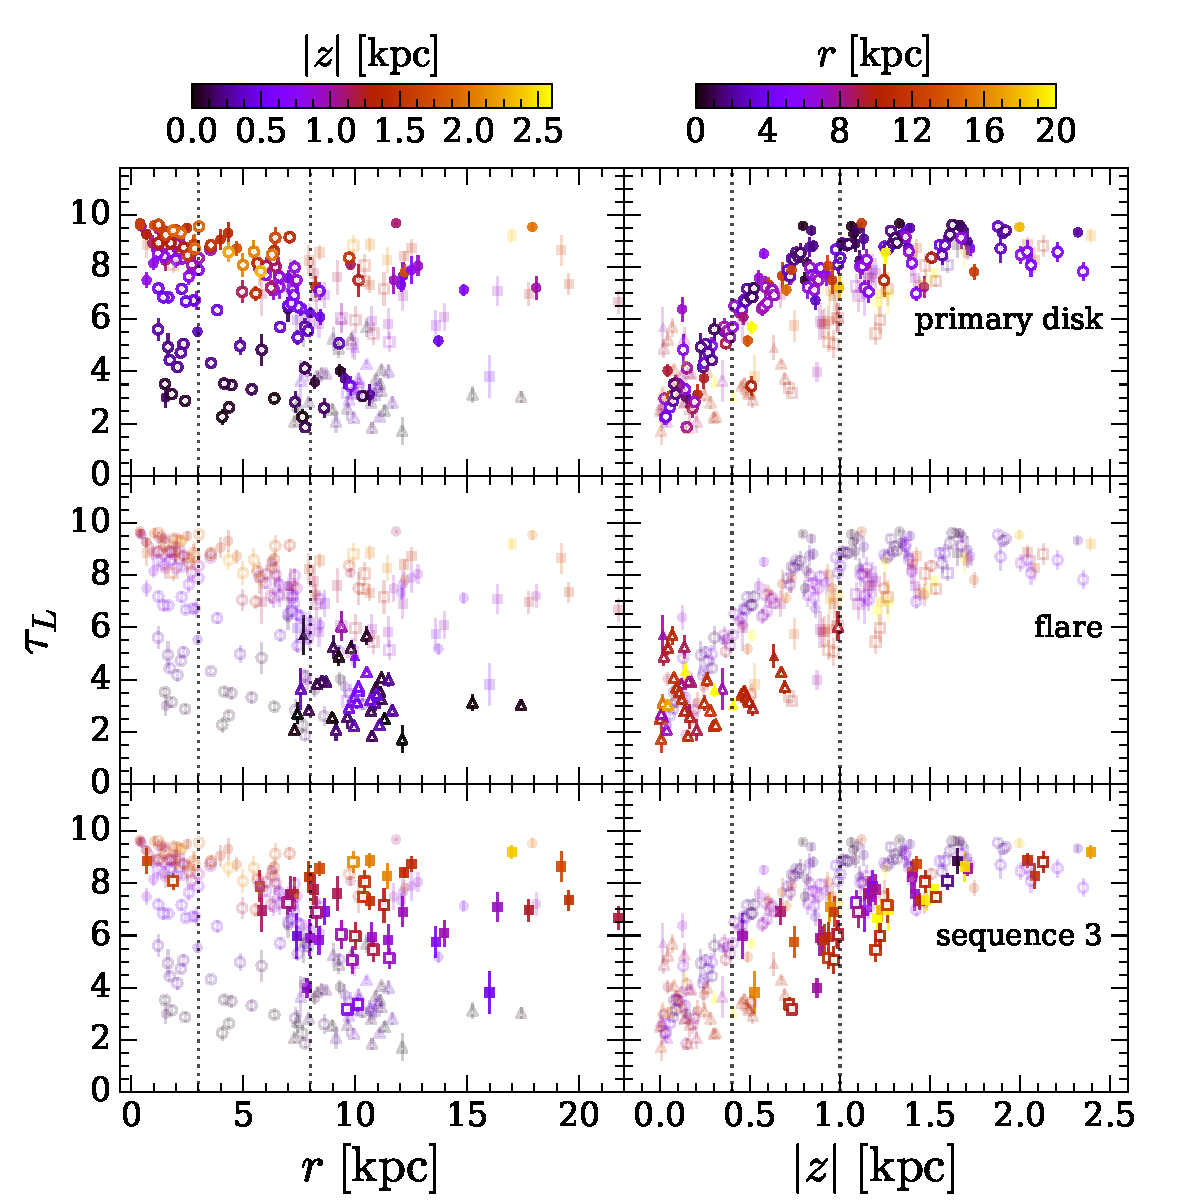
\includegraphics[width=\textwidth]{891_2/figs/MLWA_rz_all.pdf}
%%   \caption[$\tau_L$ vs
%%     ($r,|z|$)]{\fixspacing\label{891_2:fig:MLWA_rz}$\tau_L$ as a
%%     function of true radius (\emph{left}) and height
%%     (\emph{right}). On each side the points are color coded by the
%%     opposite position parameter. Open and filled circles correspond to
%%     the approaching ($r_\mathrm{proj} < 0$) and receding
%%     ($r_\mathrm{proj}\geq 0$) side of NGC 891, respectively. Vertical
%%     dotted lines correspond to the radial and vertical cuts used in
%%     \ref{chap:891_1} and Figure \ref{891_2:fig:SFH_cuts}. The three
%%     rows show the exactly the same data, but shaded to highlight the
%%     feature identified in the right-hand labels.}
%% \end{figure*}

%% Figure \ref{891_2:fig:MLWA_rz} shows the projection of our data onto the
%% $\tau_L(r,z)$ plane. The three broadly defined regions from
%% \ref{chap:891_1} are immediately obvious in the top-right
%% panel (i.e., primary disk): below \val{0.4}{kpc} all of the
%% populations are young (\val{< 6}{Gyr}), the region where $0.4 < |z|
%% \leq \val{1}{kpc}$ is a transition zone where the age generally
%% increases, and above \val{1}{kpc} the average population age
%% asymptotes to the oldest age (\val{\asim 10}{Gyr}). As described in
%% \S\ref{891_2:sec:sys_err} the specific value of $\tau_L$ at the largest
%% heights is dependent on the physical assumptions made when
%% constructing the models (i.e., the first stars in the Universe formed
%% \val{\asim 12}{Gyr} ago), but these assumptions only modulate the
%% actual value; the conclusion that the integrated light is dominated by
%% the oldest possible populations above \val{1}{kpc} is valid regardless
%% of the specific population age.

%% \citet{Xilouris99} fit a single stellar disk to broad band photometric
%% profiles of NGC 891 and find a scale height of 0.38 - \val{0.43}{kpc}
%% from $K$ to $B$ bands. In this context it is plausible that our
%% primary disk roughly corresponds to this single stellar disk. However,
%% more recent studies of NGC 891 \citep{Schechtman-Rook12,
%%   Schechtman-Rook13, Schechtman-Rook14} have refined this single-disk
%% mode to include three distinct disk components: super-thin, thin, and
%% thick with scale heights (in $K_S$ band) of 0.16, 0.47, and
%% \val{1.44}{kpc}, respectively. In this view it is likely that the
%% smooth transition from young to old ages seen in the upper-left panel
%% of Figure \ref{891_2:fig:MLWA_rz} is a result of the superposition of these
%% different disk components and thus our primary ``disk'' encapsulates
%% substructure beyond our measurement capabilities. Furthermore, the
%% primary disk also does not extend much beyond $r=\val{8}{kpc}$, which
%% is where \citet{Schechtman-Rook13} identify a truncation in their
%% super-thin disk

%% %++++++++++
%% %% {\bf MAB: Xilouris99 is a fine place to start, but I would like you to
%% %%   move on from discussing the Xilourin99 single-disk fit to the more
%% %%   sophisticated modeling from ASR (cite all 3 papers). With that in
%% %%   mind you should consider the different radial zones and how the
%% %%   flare fits in with that.

%% %++++++++++
%% %% I don't agree with your statement that above 1 kpc we are seeing the
%% %% halo as opposed to the thick disk. The points I would like to see
%% %% emphasized are that (1) there is a smooth trend of increasing age with
%% %% height that plateaus above 1 kpc. (2) At intermediate heights there is
%% %% considerable variation in age that you will then proceed to explain by
%% %% the flare and sequence-3. (3) That the 'primary disk' or sequence-1
%% %% appears to be limited primarily to the inner 8 kpc, corresponding to
%% %% the radial break of the super-thin disk seen by ASR. The thicker
%% %% component seems to be radially shorter and quite old suggesting it is
%% %% associated with the old inner disk and pseudo bulge. The thinner
%% %% portion has a range of ages. As a whole, the upper age envelop of the
%% %% 'primary disk' or sequence-1 appear to drop rapidly beyond 6 kpc.

%% %% }

%% Radial trends in $\tau_L$ reveal detailed substructure in NGC 891. The
%% top-left panel of Figure \ref{891_2:fig:MLWA_rz} confirms that, in the
%% primary disk at a given radius, older populations occupy larger
%% heights, but it is also clear that the maximum age at these large
%% heights decreases slightly with increasing radius.

%% %--------------
%% %% {\bf MAB: I agree generally with the age-radius trend except sequence-3
%% %% kind of mucks this up. Thoughts?}

%% The middle row of Figure \ref{891_2:fig:MLWA_rz} highlights the flare of NGC
%% 891. At low heights it occupies the same $\tau_L$ space as the main,
%% primary disk, but as height increases the ages stay relatively young
%% compared to the main disk. Importantly almost all of the apertures
%% belonging to this sequence exist at radii beyond \val{8}{kpc}, which
%% is one of the main reasons we identify this feature as a flared
%% extension of the star forming disk. Such a flare would be manifest as
%% an increase in scale height with radius and thus the star-forming disk
%% would extend to larger heights at large radii. Given this simplistic
%% picture, and assuming the star-forming disk extends to roughly 1 scale
%% height at all radii we can roughly estimate that at radii \val{>
%%   8}{kpc} flaring has increased the scale height by roughly a factor
%% of two (up to \val{\asim 0.8}{kpc}).

%% %% {\bf MAB: how quantitative is your scale-height estimate? This is
%% %%   nice, and if it is robust we ought to quote it in the abstract.}
%% %% ADE comment: not very robust, hence the change to ``roughly estimate''

%% The bottom row of Figure \ref{891_2:fig:MLWA_rz} shows the high-metallicity
%% ``sequence 3''. It exists only at heights above \val{0.4}{kpc} and
%% mostly beyond $r = \val{8}{kpc}$ and is made up of stellar populations
%% that are generally younger than the stars from the primary disk
%% in the same ($r,z$) locations. That said it is clear that many of the
%% apertures in sequence 3 contain a significant amount of light
%% contributed by Old population stars with the slightly lower age at large
%% heights is most likely indicative of an increased contribution from I2
%% populations.

%% %++++++++++++=
%% %% {\bf MAB: ``O population stars'' is very confusing because I read this
%% %%   as ``O stars,'' i.e., hot young stars not old DFK. So we have to be
%% %%   careful.}

%% % beyond these general trends there is evidence that at larger radii ($r
%% % > \val{\asim 8}{kpc}$) there is a separate grouping of points that
%% % occupy a younger locus than the rest of the data at similar
%% % radii. This seconday population still exhibits a general ageing of
%% % stellar population with height, but at values systematically below the
%% % main trend. Given the clumping of this younger grouping in both $r$
%% % and $z$ it is reasonable to assume that it occupies a coherent
%% % sub-structure in NGC 891. A flared disk has been suspected {\bf REF!}
%% % and would explain the presence of young stellar populations at larger
%% % heights. 

%% \subsubsection{{\Large $A_V$}}

%% \begin{figure*}
%%   \centering
%%   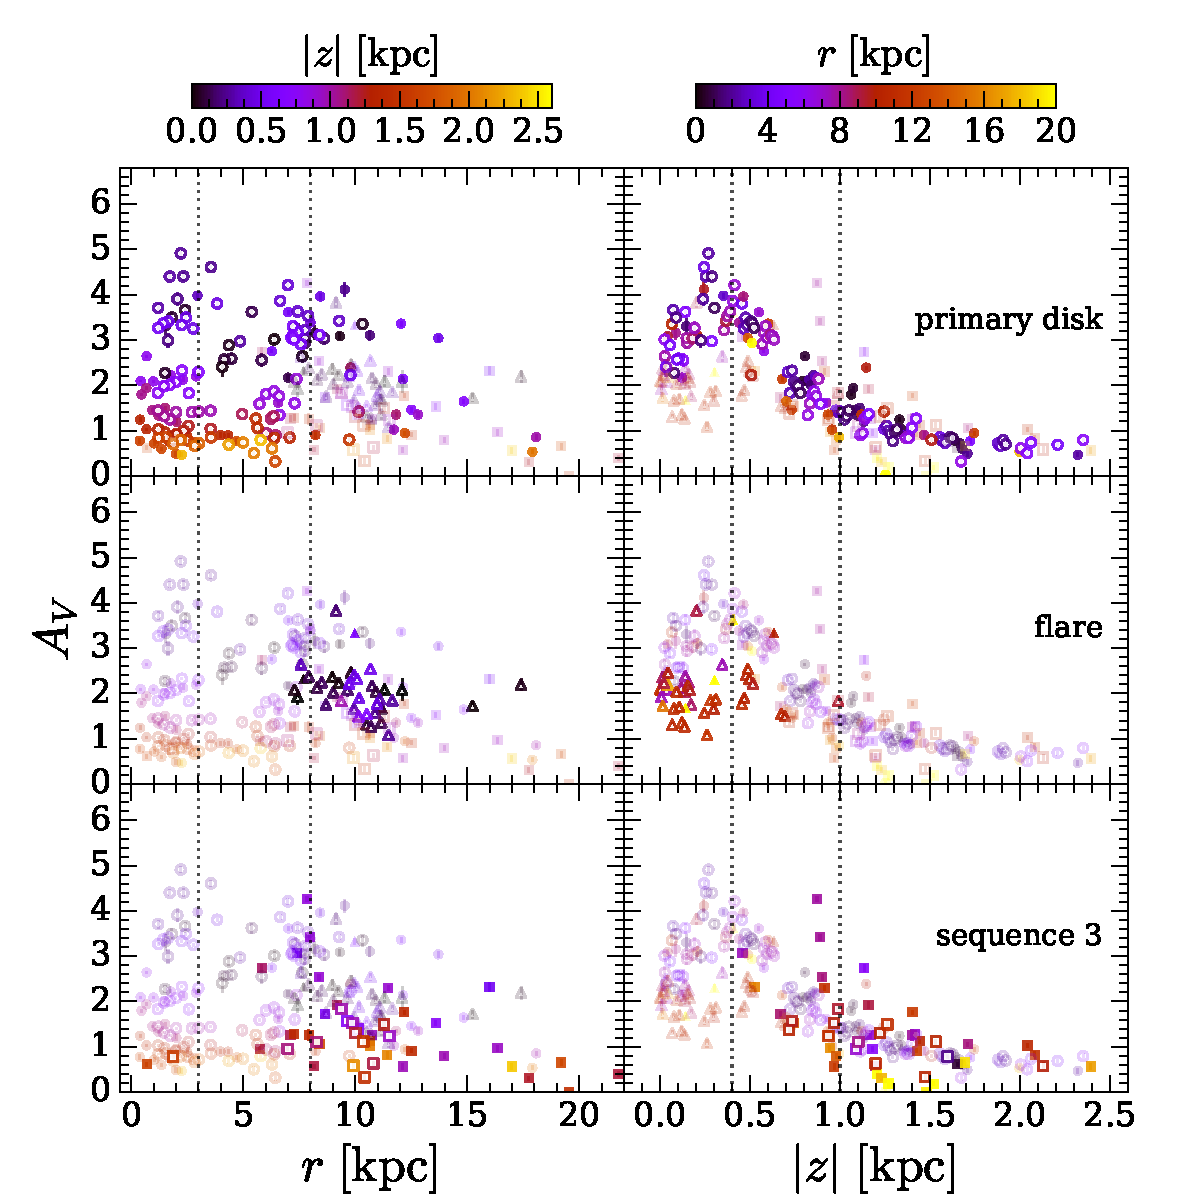
\includegraphics[width=\textwidth]{891_2/figs/AV_rz_all.pdf}
%%   \caption[$A_V$ vs ($r,|z|$)]{\fixspacing\label{891_2:fig:AV_rz}$A_V$
%%     as a function of true radius (\emph{left}) and height
%%     (\emph{right}), plotted in the same style as Figure
%%     \ref{891_2:fig:MLWA_rz}}
%% \end{figure*}

%% In Figure \ref{891_2:fig:AV_rz} the three morphological features mentioned
%% above are identified in the $A_V(r,z)$ plane. The primary disk (top
%% row) shows slightly increasing extinction with height below \val{\asim
%%   0.4}{kpc} followed by a roughly exponential decrease with height
%% above \val{\asim0.4}{kpc}. These results lend further proof to the
%% conclusion that the region below \val{0.4}{kpc} is the location of
%% current star formation, which requires regions of optically thick dust
%% and gas. Above \val{0.4}{kpc} the older stars are likely to be
%% smoothly distributed in a way that is uncorrelated with the dust. Thus
%% at the heights where old stars dominate we measure a reasonable
%% estimate of some mean extinction along a significant line of sight. At
%% low heights the dust is patchy, very dense, and correlated with
%% younger stars and so our line of sight is likely to be abruptly
%% truncated at some relatively short line of sight, and hence the stars
%% we \emph{do} see have relatively little extinction, hence the lower
%% extinction values below \val{0.4}{kpc}.

%% %----------------
%% %% {\bf MAB: Do you mean to say that $A_V(r)$ is an exponential
%% %%   function of $r$ above 0.2 kpc? Draw or fit a curve? This is the
%% %%   place to compare $A_V$ with the Balmer values. It would be
%% %%   particularly interesting to see if the different groups (primary,
%% %%   flare, seq-3) are different in this comparison. More on the
%% %%   radial trend in the next par.}
%% %% ADE: Not sure what you mean by $A_V(r)$ being exponential above 0.2 kpc.

%% %+++++++++++++++
%% %% {bf MAB: Here, concerning the down-turn at very low heights, let me
%% %%   say this differently and perhaps more plausibly. The down-turn at
%% %%   very low radii seems implausible, but we need to consider the
%% %%   transition from young to old populations seen in the previous
%% %%   figure. The older stars are likely to be smoothly distributed in a
%% %%   way that is uncorrelated with the dust. When the old stars dominate
%% %%   at larger heights we get a reasonable estimate of some mean
%% %%   extinction along a significant line of sight. At low height, since
%% %%   the dust is patchy, very dense, and correlated with younger stars,
%% %%   our line of sight is likely to be abruptly truncated at some
%% %%   relatively short line of sight, and hence the stars we do see have
%% %%   relatively little extinction. This should correspond to the LOS
%% %%   depths, which is why it would be nice to show the trend with height
%% %%   to refer back to here.

%% %% }

%% Above \val{0.4}{kpc} the general decline in $A_V$ is consistent with
%% the simple morphological view of exponentially decreasing surface
%% density in edge-on galaxies. The rate of decline shown in Figure
%% \ref{891_2:fig:AV_rz} indicates the scale height of attenuating material is
%% \val{\asim 0.6}{kpc}, which is significantly larger than either
%% \citet{Xilouris99} or \citet{Schechtman-Rook12}, who find a vertical
%% dust scale height of 0.3 and \val{0.24}{kpc} in the $V$ and $K_S$
%% bands, respectively. It is important to note, however, that both of
%% these studies find a wavelength dependence on extinction that is
%% steeper than the model of \citet{Charlot00} used in our model galaxies
%% (see \S\ref{891_2:sec:extinction}). Our prescription of extinction therefore
%% requires larger normalization values ($A_V$) to achieve the same level
%% of extinction which makes direct comparison of our data to the
%% conclusions of \citet{Xilouris99} or \citet{Schechtman-Rook12}
%% difficult.

%% %++++++++++++++
%% %% {\bf MAB: This is nice. Finish the analysis, include the results from ASR,
%% %% use all of the dust scale-heights for the different bands and let's
%% %% see if we can work this out. Show a model curve.}

%% The middle row of Figure \ref{891_2:fig:AV_rz} shows that flared extension
%% of the primary disk has systematically lower extinction than the main
%% disk. In a flared disk with a roughly constant total dust fraction an
%% increase in scale height at large radii (i.e., the flare) would cause
%% the dust surface density to decrease at these larger radii, which is
%% consistent with the lower values of $A_V$ seen in the data
%% corresponding to the flare. A paucity of data points above $z =
%% \val{0.4}{kpc}$ and within $r = \val{8}{kpc}$ makes it difficult to
%% determine vertical or radial trends in the flare's extinction, but to
%% 1st order these trends appear to be constant.

%% %--------------
%% %% {\bf MAB: My read of Figure \ref{891_2:fig:AV_rz} is that there is evidence
%% %%   for a decrease in extinction at lower heights at larger radii.}
%% %% ADE: I don't agree with this

%% Sequence 3 does not stand out very much in the $A_V(r,z)$ planes. It
%% shows extinction values that are generally consistent with the other
%% morphological features that exist at smaller radii, albeit with more
%% scatter (bottom right panel of Figure \ref{891_2:fig:AV_rz}).

%% %++++++++++++++++++
%% %% {\bf MAB: My read of Figure \ref{891_2:fig:AV_rz} is that it is hard to
%% %%   conclude on seq-3 except to see that it appears to have much more
%% %%   variation in $A_V$ with height, although it does not appear to be
%% %%   inconsistent at a given height with its counterpart populations at
%% %%   smaller radius. I think you say much of this and I don't think it is
%% %%   important to emphasize that seq-3 ``occupies a locus with lower
%% %%   extinction than either the star forming disk or the flare'' because
%% %%   I think this can be explained by height.}

%% \subsubsection{{\Large $Z_L$}}

%% \begin{figure*}
%%   \centering
%%   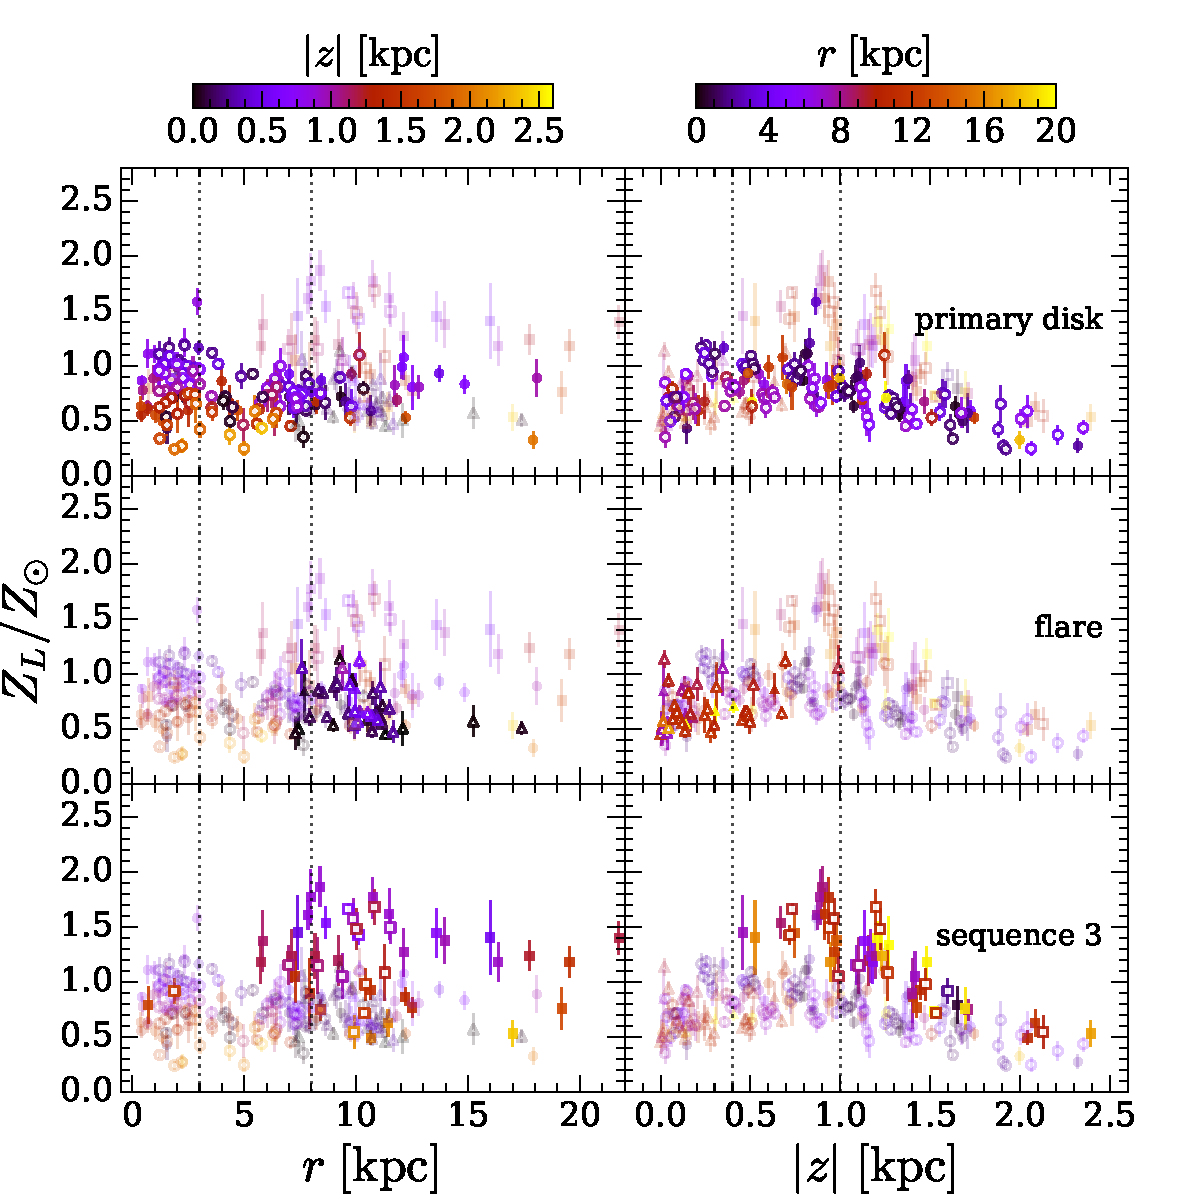
\includegraphics[width=\textwidth]{891_2/figs/MLWZ_rz_all.pdf}
%%   \caption[$Z_L$ vs
%%     ($r,|z|$)]{\fixspacing\label{891_2:fig:MLWZ_rz}$Z_L$ as a function
%%     of true radius (\emph{left}) and height (\emph{right}), plotted in
%%     the same style as Figure \ref{891_2:fig:MLWA_rz}}
%% \end{figure*}

%% Finally, Figure \ref{891_2:fig:MLWZ_rz} shows $Z_L$ as a function of
%% location in NGC 891 and highlights the discriminatory power of
%% metallicity in identifying the three morphological features mentioned
%% above. The primary disk shows slightly negative correlations
%% between metallicity and both radius and height (top panel). This view
%% is consistent with measurements from the Milky Way \citep{Bovy12,
%%   Hayden14} and with the conclusions of
%% \ref{chap:891_1}. This also reaffirms the idea that stars at
%% large heights are formed from pristine gas at early times (as shown in
%% Figure \ref{891_2:fig:MLWA_rz}.

%% In the middle row of Figure \ref{891_2:fig:MLWZ_rz} shows strong evidence
%% that the flare identified in previous sections comes from the same
%% underlying distribution as the primary disk. At all radii and heights
%% in the $Z_L(r,z)$ plane the flare points are essentially
%% indistinguishable from those of the primary disk. The flare exists in
%% a different ($r,z,A_V$) location, but it's ages and, importantly,
%% metallicity are consistent with the same populations seen in the disk.

%% %% {\bf MAB: don't push too hard on Z for young-age pops.}  

%% Sequence 3 is perhaps most visible as a high-metallicity sequence in
%% the $Z_L(r,z)$ planes, as shown in the bottom row of Figure
%% \ref{891_2:fig:MLWZ_rz}. At all radii and heights it occupies a locus that
%% has larger values of $Z_L$ than either the primary disk or the flare
%% (which are the same in terms of metallicity). Despite these high
%% values it still follows a general trend of decreasing metallicity with
%% height and radius, which suggest that whatever evolutionary mechanisms
%% cause the trends in the disk also affect the large radii and heights
%% occupied by sequence 3.

%% %% These results, coupled with those shown in Figure \ref{891_2:fig:MLWA_rz}
%% %% yield a possible explanation for the presence of sequence 3. This
%% %% sequence is distinct in both age and metallicity from the primary disk
%% %% and flare

%% %+++++++++++++++
%% %% {\bf MAB: Isn't $Z_L(r,z)$ a volume not a plane? Maybe another way to
%% %%   say your last point which also ties in to the flare is that we are
%% %%   seeing a population sequence at large radii and large heights that
%% %%   is distinct in both age and metallicity from what looks to be the
%% %%   old thick disk seen over a range of radii. It may be a temporal
%% %%   extension of the flare seen at younger ages, i.e., stars that formed
%% %%   in a flared disk at an intermediate era.}

%% %% ADE: This is nice, but how does the temporal fare extension picture
%% %% jive with \emph{higher} metallicities than the younger flare?

%% % The average metallicity appears to increase slightly with
%% % height up to \val{1}{kpc} where it abruptly begins to decrease with
%% % increasing height. We note, however, that the apparant increase up to
%% % \val{1}{kpc} is driven mostly by a few super-solar points between 0.4
%% % and \val{1}{kpc} and at large radii. As we have seen above, the radial
%% % structure of NGC 891 is highly non-uniform and we therefore caution
%% % that these few points are probably not representative of a global
%% % trend. Thus ignoring these super-solar points the average metallicity
%% % is relatively constant below \val{1}{kpc}, at which point it decreases
%% % with height. This general trend is qualitatively consistent with
%% % results from the Solar cylinder in the Milky Way
%% % \citep{Hayden15,Bovy12} and supports the theory that large heights are
%% % primarily populated by old stars that formed from pristine gas.

%% % Much like $\tau_L$ and $A_V$ there appears to be a second order,
%% % bi-modal $Z_L$ distribution in NGC 891. Starting at $z = \val{\asim
%% %   0.4}{kpc}$ there is a cluster of apertures with super-solar
%% % metallicities that follow the same general trend as the global average
%% % (i.e., decreasing with radius above \val{1}{kpc}), but at a higher
%% % metallicity. All of these high-$Z_L$ apertures exist at radii beyond
%% % \val{8}{kpc}, which suggests they belong to the same sub-structure
%% % identified in $\tau_L$. Under the assumption that this sub-structure
%% % is a flared disk the presence of high metallicity stellar populations
%% % indicate that this disk is likely the site of a recent epoch of star
%% % formation, a claim supported by the systematically lower ages see in
%% % Figure \ref{891_2:fig:MLWA_rz} for the same structure.

\subsection{Star Formation History}
\label{891_2:sec:SFH}
\begin{figure*}
  \centering
  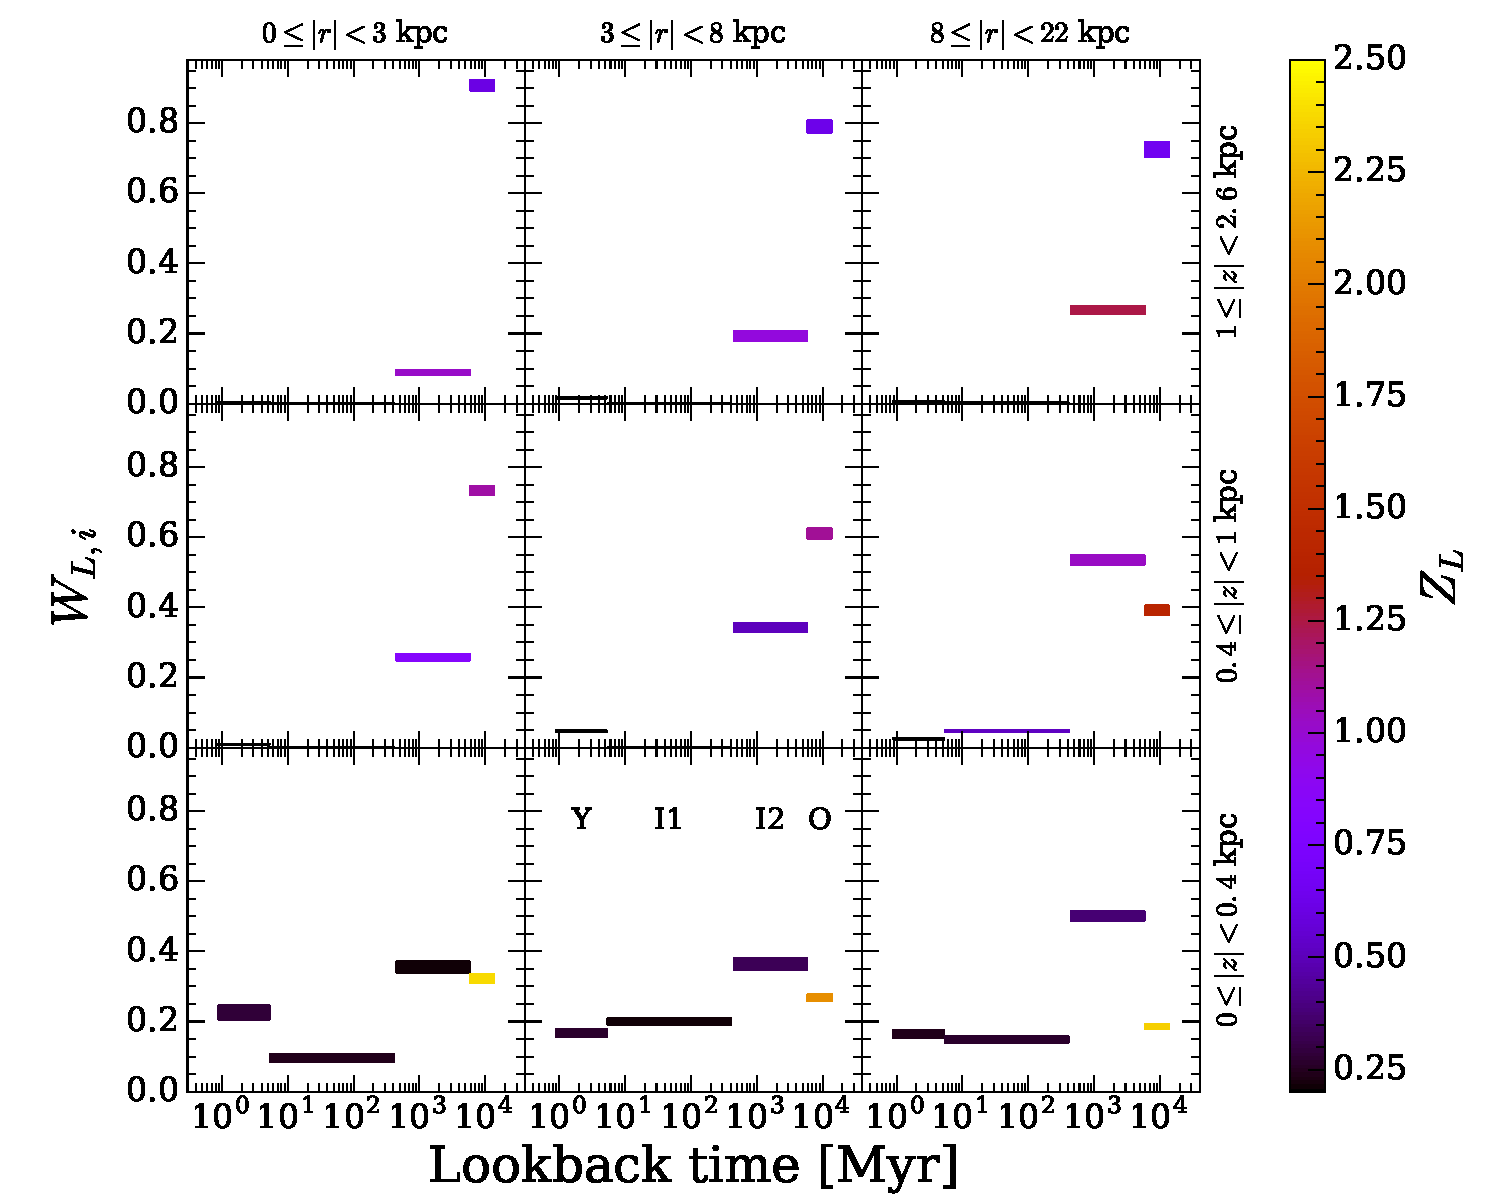
\includegraphics[width=\textwidth]{891_2/figs/SFH_cuts.pdf}
  \caption[SSP light weights in ($r,|z|$)
    grid]{\fixspacing\label{891_2:fig:SFH_cuts}Fractional light-weight
    (Equation \ref{891_2:eq:light_weight}) for each DFK age bin as a
    function of radius and height. The radial and height bins shown
    are the same as used in \ref{chap:891_1} and highlight the
    different components of NGC 891 described in the text. The
    horizontal extent of each bar spans the range of ages covered by
    each SSP and the vertical width of each bar corresponds to the
    fitting uncertainty of each weight computed using the same method
    detailed in \S\ref{891_2:sec:fit_err}. Each weight is color coded
    by the average $Z_L$ in the particular ($r,z$) bin.  }

\end{figure*}

A primary benefit of full-spectrum SSP fitting is that it allows us to
fit and measure the star formation history (SFH) for every aperture in
our data set. As discussed in \S\ref{891_2:sec:sys_err} the mean,
light-weighted age ($\tau_L$) is a convenient proxy for SFH, but
requires an assumed SFH for the models used to fit our galaxy data. To
avoid these assumptions we can examine the integral of the SFH
multiplied by the flux of each SSP, which is identical to the
light-weights found during SSP fitting (see
\S\ref{891_2:sec:SSP_method} and Equation \ref{891_2:eq:MLWA}). Figure
\ref{891_2:fig:SFH_cuts} shows these values in the same grid of radius
and height used in \ref{chap:891_1} (although now the radius values
are the true, cylindrical values a la \S\ref{891_2:sec:LOS}). From
these data we can see the same general trend found in \ref{chap:891_1}
and above: younger populations predominantly exist below
\val{0.4}{kpc}. There are also small contributions from young
populations above \val{0.4}{kpc} at the largest radii, which confirms
the idea that NGC 891 built up from a superposition of flared disks
with increasing ``flare radii''.

Above \val{0.4}{kpc} (and even below this for $r < \val{8}{kpc}$) the
I2 populations contribute more to the total light at larger radii,
with a corresponding decrease in the contribution from Old
populations. This trend is broadly consistent with an inside-out view
of star formation in NGC 891. Such a formation scenario (which we also
see in \ref{chap:891_1}) predicts a higher fraction of young and
intermediate aged stars at large radii, exactly as seen in Figure
\ref{891_2:fig:SFH_cuts}.

%% Further evidence for a flare can be seen in the fact that I2
%% populations (see Table \ref{891_2:tab:dfk}) contribute more to the total
%% light at larger radii, with a corresponding decrease in contribution
%% from O populations. This picture provides further insight into
%% secondary morphological feature (i.e., flare) identified in
%% \S\ref{891_2:sec:rz}, specifically that, while it shows the same positive
%% age/height gradient seen in the main primary disk, its oldest
%% stellar populations are at most \val{\asim5.7}{Gyr} old (i.e., the old
%% limit of the I2 DFK bin). 

%% {\bf MAB: I am not sure I followed this paragraph. It is not clear to
%% me that the trends in O and I2 DFKs in the 6 bins for $z>0.4$ kpc
%% are consistent with flares. What if the thick disk is simply
%% younger at larger radii. Maybe I am missing something?}

%% Despite this decrease O populations are still the primary source of
%% light for all radii at heights above \val{1}{kpc}. This observation is
%% consistent with the conclusions from \S\ref{891_2:sec:rz} that any flare in
%% NGC 891 extends up to \val{\asim 1}{kpc}, but not much beyond this
%% height.

%++++++++++++++++++++++
%% {\bf MAB: In this discussion I think we need to be careful what we
%%   mean by flare. For example, the Martig+14 simulations have all of
%%   the mono-age populations flaring, just at different radii, inside
%%   out. So when we say flare, do we mean only the Y and I1 pops?}

%% ADE: Agree, the increase in I2 with radii can more simply be
%% explained as inside out formation, which is consistant with paper1

Finally, the metallicity color-coding in Figure
\ref{891_2:fig:SFH_cuts} is consistent with the enrichment history
presented in \S\ref{891_2:sec:tZ}. The youngest populations (which
only contribute appreciable light at low heights) are very metal poor
because they are formed from pristine material that has recently
fallen onto the disk of NGC 891 (see also Figure
\ref{891_2:fig:MLWZ_rz_cut}). At these low heights the most metal-rich
population is the Old population, and indeed it is this population
that has the largest value of $Z_L$ anywhere in NGC 891. This suggests
that the Old populations at low heights correspond to the youngest
limit of the Old DFK age bin, which is exactly the age of ``peak
metallicity'' discovered in \S\ref{891_2:sec:tZ} (\val{\asim 6}{Gyr}).

We also see that the metallicity of the Old population decreases with
height (at all radii) while the metallicity of the younger populations
increases with height. Once again, this beautifully illustrates the
enrichment history presented above; the Old population formed during
the ``closed-box'' period in NGC 891's history, where older stars
(i.e., stars at larger heights) formed from pristine gas. Star
formation more recent that \val{6.6}{Gyr} (i.e., anything besides the
Old population), however, occurred during a time when metal-poor gas
from outside of NGC 891 caused \emph{younger} stars (i.e., those at
lower heights) to have decreased values of metallicity.

%% At first glance the $Z_L$ values shown in Figure
%% \ref{891_2:fig:SFH_cuts} seem counterintuitive; at the lowest heights
%% the largest values of metallicity occur in the oldest SSPs and the I2
%% SSPs show metallicity values that increase with height. The first
%% trend is likely due to the positive correlation between age and
%% metallicity identified at low heights in
%% \S\ref{891_2:sec:fit_err}. Indeed, below \val{0.4}{kpc} the Y and I1
%% SSPs are very metal poor, while I2 and O have higher metallicities,
%% consistent with the degeneracies seen at these low heights. In other
%% words, the high metallicity in Old populations below \val{0.4}{kpc} is
%% likely a result of fitting degeneracies and perhaps not an accurate
%% representation of the physical picture in these regions.

%% %++++++++++++
%% %% {\bf MAB: This hi-Z O population at low heights has me concerned.  Do
%% %%   we think this is real or an artifact of our fitting?  It could be
%% %%   real if there is indeed an old, metal-rich thin disk, although one
%% %%   wonders why I2 is so metal poor at the same height. Since we have
%% %%   supposedly corrected for projection and have everything in the right
%% %%   radial bins it would be hard to invoke the older stars being from
%% %%   smaller radii where metallicity is higher. So this is why I wanted
%% %%   to see mass-weighted plots.}

%% To explain the trend in increasing metallicity with height seen in the
%% I2 populations we invoke the flare identified in this and previous
%% sections. Recent star formation in the ``normal'' primary disk (i.e.,
%% not the flare) does not extend much above \val{\asim 1}{kpc} and any
%% stars at these large heights are likely to be old and metal poor. The
%% flare, on the other hand, as shown above, exhibits recent (in this
%% case \val{\asim 6}{Gyr} ago) star formation at heights above
%% \val{1}{kpc}. Thus, as height increases the fraction of I2 stars that
%% belong to the flare (and therefore have higher metallicities)
%% increases and the average $Z_L$ in the I2 bin increases. This
%% interpretation is consistent with the morphological picture present in
%% \S\ref{891_2:sec:rz} and allows us to actually infer something about the SFH
%% in NGC 891. As shown in Table \ref{891_2:tab:dfk} the I2 bin spans roughly
%% \val{5}{Gyr} which is a significant fraction of the total age of NGC
%% 891 (assumed here to be \val{12}{Gyr}). In the primary disk I2 stars
%% are considered ``old'', have low metallicities, and were therefore
%% likely formed at the older end of the I2 bin (\val{\asim 6}{Gyr}). At
%% larger heights, however, light from the flare dominates in all but the
%% oldest SSP bin, and thus the I2 DFK bin represents a fundamentally
%% different population of stars; those that formed near the young limit
%% of the I2 bin (i.e., \val{\asim 500}{Myr}) and therefore have higher
%% metallicities (as seen in Figure \ref{891_2:fig:SFH_cuts}).

%----------------
%% {\bf MAB: I don't understand the first sentence. Do you mean the
%%   positive metallicity gradient with radius for I2 at each height? Or
%%   do you mean the positive gradient in WL with radius for all heights?
%%   Or ...?  I would drop the claim that stars above 1 kpc are
%%   ``primordial halo stars that are coeval with NGC 891.'' You just
%%   don't know that. If you want to assume it, and then see what follows
%%   that's a different matter. In any evet I would not assume they are
%%   part of the halo.

%% I'm not sure I buy this and what follows: ``Thus, as height increases
%% the fraction of I2 stars that belong to the flare (and therefore have
%% higher metallicities) increases and the average $Z_L$ in the I2 bin
%% increases.'' Again, why is this all due to the flare as opposed to an
%% outer thick disk what has different age and metallicity properties
%% because of some inside-out formation?

%% ADE: I see what you're saying about ``why flare and not just a thicker
%% disk'', but I really think that Figure \ref{891_2:fig:MLWA_rz} tips the
%% scales in favor of a flare. Basically, the fact that our ``flare''
%% only exists at large radii rules out a thicker disk. Right? 
%% }


%% Given the data shown in Figure \ref{891_2:fig:MLWA_rz} we conclude that the
%% majority of the flare stars are coveal with the main star forming
%% disk, which suggests the flare is simply an increase in scale height
%% (of both gas and stars) at larger radii and not representative of a
%% fundamentally different population. Figure \ref{891_2:fig:MLWZ_rz}, however,
%% suggests that the flare stars \emph{do} occupy a location in parameter
%% space separate from the primary disk; one of higher
%% metallicity. The true picture is likely somewhere in the middle;
%% what's certain is that stars in the ``flare'' have a similar SFH as
%% the main primary disk but formed from gas with a higher
%% metallicity than that found towards the inner regions of NGC 891.

%++++++++++++++++++
%% {\bf MAB: We should talk about this. I don't have my head wrapped
%%   around it so I am not yet onboard.}

%% ADE: Ya, I don't get it either. Not sure what I was thinking
%% here. Figure 21 clearly shows that the ``flare'' stars have the
%% same metallicity as the primary disk. Just took it out for now.

%% The first order effect that we are seeing is that there is a positive
%% age gradient with height above the mid-plane, consistent with
%% qualitative expectations.

%% Lower metallicity (sub-solar) models appear to give flatter age
%% profiles at large height, which is what we would expect.  In contrast,
%% models with solar and above metallicity yield lower ages at the
%% largest heights relative to mid-latitude values, i.e., the ages roll
%% over a bit at large heights.  This may very well be a systematic
%% effect if indeed the high-latitude population is intrinsically
%% low-metallicity since forcing higher metallicity increases
%% line-strength which would then have to be compensated for in the model
%% fitting with younger ages. On the other hand, we need to be careful
%% (a) not to over-interpret small changes in age at large ages (where
%% there is little leverage in the models; and (b) not to make
%% conclusions based on our initial assumptions.

%% We don't see much correlation of the optical depth with the adopted
%% metallicity of the SPS models. We should quantify this, but it is
%% reassuring. This means, for example, that metallicity and age are
%% largely keying off the line-strengths and not the continuum spectral
%% shape, but we should check this in detail--for example, by looking at
%% correlations between age vs $A_V$ in residuals about the mean at a
%% given height.

%% There do appear to be radial trends in the sense that the outer disk
%% is younger, and younger at a given height, although this trend has not
%% been isolated from metallicity effects (e.g., perhaps the outer disk
%% is also more metal poor, as seen in the Milky Way).

%% We also have not looked carefully to determine if the age gradients
%% are symmetric with radius on either side of the galaxy.
